\section{Description of the Project}
Our goal for this project is to visualize word embeddings by avoiding the clutters caused by too many data points. 
Our core idea for the approach is to collapse the data points into clusters and annotate with emoji to summarize the cluster.
Figure~\ref{fig:cluster_network} shows the example output of our visualization. 

\begin{figure}[htb]
 \centering
     {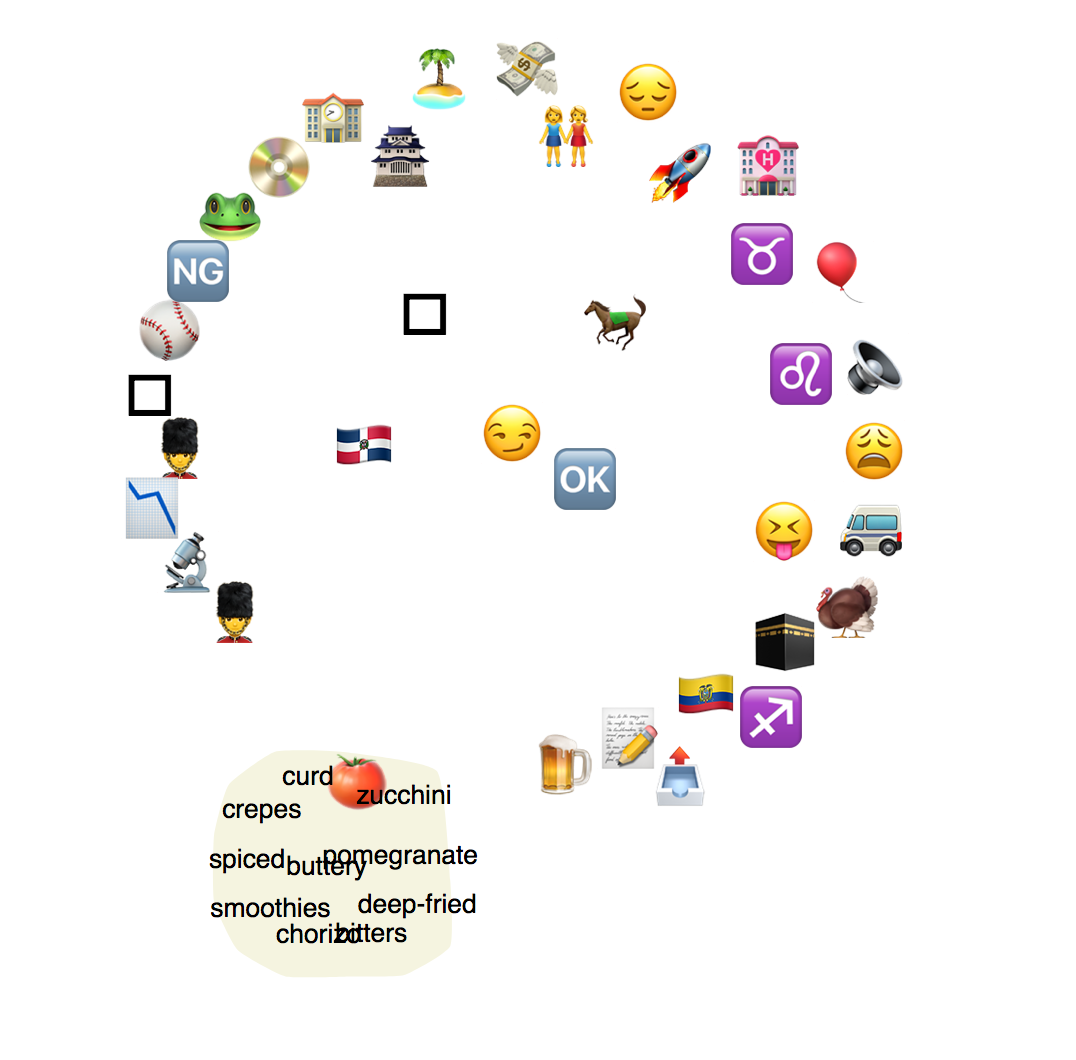
\includegraphics[width=0.68\linewidth]{figures/clustered_network.png}}
    \vspace{-1ex}
     \caption{The visualization of word embeddings using clustered network and emojis.}
\label{fig:cluster_network}
\end{figure}

\begin{figure}[htb]
 \centering
     {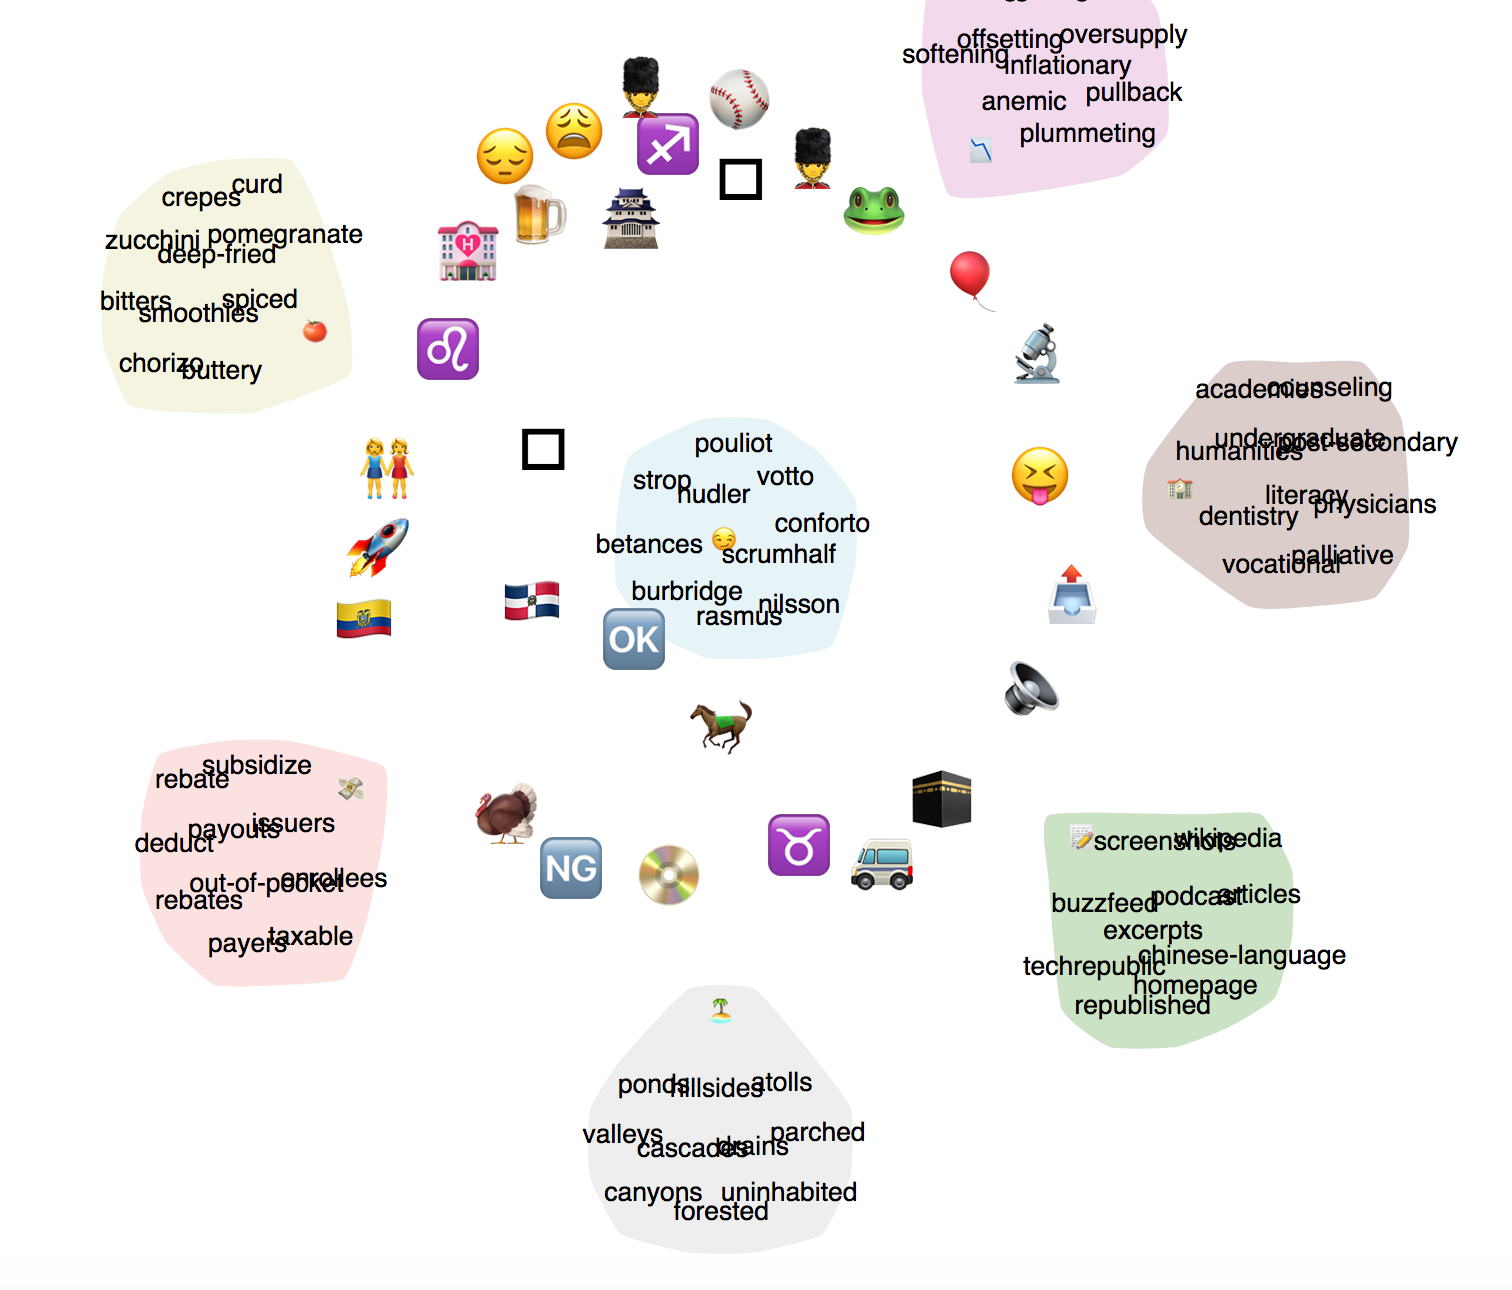
\includegraphics[width=0.68\linewidth]{figures/clustered_network_opened.png}}
    \vspace{-1ex}
     \caption{An example of expanding clusters after clicking on emojis.}
\label{fig:cluster_network_opened}
\end{figure}

Our approach for constructing the visualization is as follows:
\begin{enumerate}
 \item Train a word embedding using a raw corpus. 
 \item Run $k$-means \cite{lloyd1982least} on the word embedding space and obtain clusters
 \item Assign an emoji to each cluster
 \item Visualize the clusters using D3.js \cite{Bostock:2011:DDD:2068462.2068631}
\end{enumerate}
For the number of clusters $k$, we empirically set $k = \{40, 50\}$. 
We only show the top 10 nearest neighboring words to the centroid to avoid the visualization clutter. This issue is further discussed in Section~\ref{sec:discussion}.

\subsection{Annotation of Clusters with Emojis}
Searching for a right word to represent the cluster requires external linguistic resources e.g., WordNet and a sophisticated method e.g., hypernym prediction. 
However, humans are good at associating multiple words and capture the abstract meaning form a picture.  
%When a human look at emoji, one connects with various possible concepts. 
For example, when one looks at the tomato emoji (🍅), the possible association of this words are ``tomato'', ``vegetable'', ``food'', or even ``object''. 
Therefore, we decide to use emojis to represent the clusters. 

Another motivation of using emojis instead of words is the ``Picture superiority effect'' (e.g., \cite{doi:10.1162/jocn.2010.21464}) i.e., humans are better remembering pictures than words. 
Assuming that the annotation of clusters is the most crucial component to summarize word embeddings, we use emojis to represent the clusters.  

To assign an optimal emoji $e_c$ to each cluster $c$ with centroid vector $v_c$, assume we have a set of emoji and its text description $t$. 
We compute the mean word vector $v_t$ of each word $w_i$ in a given emoji description $t = \{w_1, w_2, ..., w_n\}$ with length $n$ out of all set of emoji descriptions $T$, i.e.,
\begin{equation}
 e_c =  \text{argmax}_{t \in T} \text{cos\_sim}(v_c, v_t)
\end{equation}
where 
\begin{equation}
 v_t = \frac{\sum_{i = 1}^{n} w_i}{n}. 
\end{equation}

Word vectors are trained by Skip-gram with negative sampling \cite{NIPS2013_5021} using 1 million sentences of English news articles from Leipzig corpora collection \cite{Goldhahn12buildinglarge}. We set the word vector dimension as $100$. 
Emojis are obtained from dataset built by \cite{eisner-EtAl:2016:SocialNLP}. 


\subsection{Interaction}
To let the users dive deeper into further details of clusters, users can click on emojis to ``drill-down'' \cite{Elmqvist:2010:HAI:1749404.1749525} the cluster and look into the nearest neighboring words in terms of the centroid in the cluster.
However, even when we collapse words into each cluster, there are still overlapping words as shown in Figure~\ref{fig:cluster_network_opened}. 
To solve this issue, we further made each cluster draggable and used forced layout to let users resolve the overlapping words. 
The core part of the D3.js code is referred from \url{http://bl.ocks.org/GerHobbelt/3071239}.

%\subsection{Force Layout}
%To solve the problem of overlapping texts, we also use force layout in D3.js to let the texts and emojis move and draggable. 
